\hypertarget{_pixel_8h}{
\section{Pixel.h File Reference}
\label{_pixel_8h}\index{Pixel.h(114)@{Pixel.h(114)}}
}


\subsection{Detailed Description}
Declaration of class \hyperlink{class_pixel}{Pixel}. 



Definition in file \hyperlink{_pixel_8h-source}{Pixel.h}.

{\tt \#include \char`\"{}Colorspace.h\char`\"{}}\par
{\tt \#include $<$Magick++.h$>$}\par


Include dependency graph for Pixel.h:\nopagebreak
\begin{figure}[H]
\begin{center}
\leavevmode
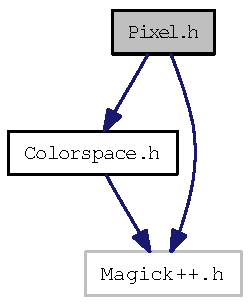
\includegraphics[width=77pt]{_pixel_8h__incl}
\end{center}
\end{figure}


This graph shows which files directly or indirectly include this file:\nopagebreak
\begin{figure}[H]
\begin{center}
\leavevmode
\includegraphics[width=408pt]{_pixel_8h__dep__incl}
\end{center}
\end{figure}
\subsection*{Data Structures}
\begin{CompactItemize}
\item 
class \hyperlink{class_pixel}{Pixel}
\begin{CompactList}\small\item\em Information about an image pixel. \item\end{CompactList}\end{CompactItemize}
